\documentclass[a4paper,cs4size]{BHCexam}
%\documentclass[a4paper,cs4size,answers]{BHCexam}

\usepackage{multicol} % 分栏
\usepackage{hyperref}
\pagestyle{fancy}
\fancyfoot[C]{\kaishu \small 第 \thepage 页 共 \pageref{lastpage} 页}
%\fancyhead[L]{\includegraphics[width=2cm]{qrcode.png}}
\title{电路习题课1}
%\subtitle{数学文科试卷}
%\notice{满分150分, 120分钟完成, \\	允许使用计算器,答案一律写在答题纸上.}
%\author{Gavin Chen}
%\date{\today}

\begin{document}
\maketitle
\begin{groups}
    \group{}{补充知识}
    电阻率(resistivity)是用来表示各种物质电阻特性的物理量。在温度一定的情况下,材料的电阻为:
    $$R=\rho  \frac{L}{S}$$
    其中的$\rho$就是电阻率,$L$为材料的长度, $S$为材料的横截面积。需要注意的是:
    \begin{itemize}
        \item 电阻率和电阻是两个不同的概念。
        \item 电阻率$\rho$不仅和导体的材料有关,还和导体的温度有关。
    \end{itemize}

    \vspace{3cm}
    \group{}{例题}
    %\zihao{-4}
    \begin{questions}[]

        \question[5]已知某导体单位体积内的自由电荷数为$n$,自由电荷的定向移动速度为$v$,自由电荷的电荷量为$q$,导体的横截面积为$S$。
        试证明电流的微观表达式:$I=nSqv$
        \begin{figure}[htb]
            \flushright
            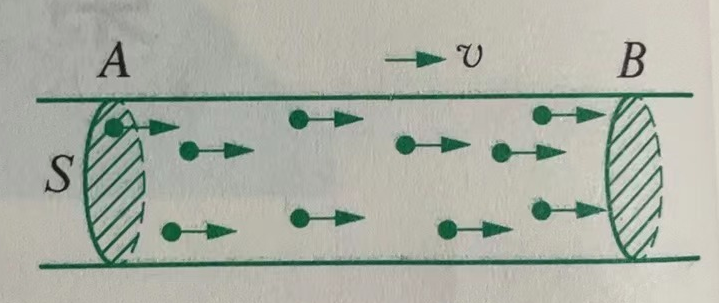
\includegraphics [scale=0.25,trim=0 0 0 0]{./image/physics_circuit1_1.png}
            % \caption{图名}
            \label{fig:fig_circuit1_1}
        \end{figure}
        \vspace{3cm}

        \question[5] 一粗细均匀的镍铬丝,截面直径力$d$,电阻为$R$。把它拉制成直径为$\frac{d}{10}$的均匀细丝后,
        它的电阻变为(\quad\quad\quad)。
        \fourchoices{$\frac{R}{1000}$}
        {$\frac{R}{100}$}
        {$100R$}
        {$10000R$}
        \vspace{1.5cm}

        \question[5] (多选)如图所示,$R_1$和$R_2$是材料、厚度相同、表面为正方形的导体板,但$R_1$的尺寸比$R_2$的尺寸大,
        在导体两端加相同的电压,通过两导体的电流方向如图所示,则下列说法中正确的是(\quad\quad\quad)。
        \fourchoices{$R_1$中的电流小于$R_2$中的电流}
        {$R_1$中的电流等于$R_2$中的电流}
        {$R_1$比$R_2$中自由电荷定向移动的速率大}
        {$R_1$比$R_2$中自由电荷定向移动的速率小}
        \begin{figure}[htb]
            \flushright
            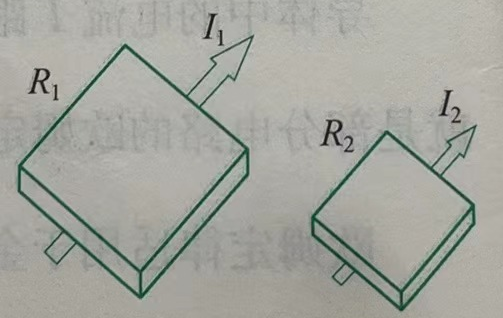
\includegraphics [scale=0.25,trim=0 0 0 0]{./image/physics_circuit1_3.png}
            % \caption{图名}
            \label{fig:fig_circuit1_3}
        \end{figure}
        \vspace{2.5cm}

        \question[5] (多选)研究某导体的伏安特性曲线,通电后其电流$I$与所加电压$U$的变化图线如图所示,
        $P$为图线上一点,$PQ$为$U$轴的垂线,$PM$为$I$轴的垂线,则下列说法中正确的是(\quad\quad\quad)。
        \fourchoices{随着所加电压的增大,该电阻的阻值增大}
        {随着所加电压的增大,该电阻的阻值减小}
        {对应$P$点的电阻值$R=\frac{U_1}{I_2}$}
        {对应$P$点的电阻值$R=\frac{U_1}{I_1-I_2}$}
        \vspace{-4.5cm}
        \begin{figure}[htb]
            \flushright
            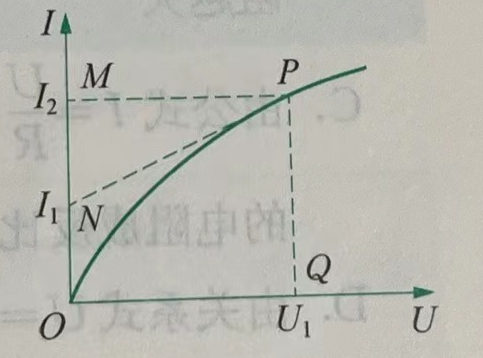
\includegraphics [scale=0.4,trim=0 0 0 0]{./image/physics_circuit1_2.png}
            % \caption{图名}
            \label{fig:fig_circuit1_2}
        \end{figure}
        \vspace{2.5cm}

        \question[5] 关于欧姆定律,下列说法中不正确的是(\quad\quad\quad)。
        \fourchoices
        {由关系式$R=\frac{U}{I}$可知,导体的电阻跟导体两端的电压成正比,跟导体的电流强度成反比}
        {关系式$R=\frac{U}{I}$表明使导体通过一定的电流所需的电压越高,则导体的电阻越大}
        {由公式$I=\frac{U}{R}$可知,导体中的电流强度跟导体两端的电压成正比,跟导体的电阻成反比}
        {由关系式$U=IR$可知,对于一个确定的导体来说,通过的电流越大,那么导体两端的电压也越大}
        \vspace{1.5cm}

        \question[5] 某导线的电阻为$160\Omega$,将它对折起来使用,它的电阻变为\underline{\quad\quad\quad\quad}$\Omega$,
        如果将它均匀地拉长到原来的$2$倍,则它的电阻为\underline{\quad\quad\quad\quad}$\Omega$。
        \vspace{1.5cm}

        \question[5] 已知电子的电量为$e$,若氢原子的核外电子绕核做半径为$r$的匀速圆周运动,线速度大小为$v$,
        则电子的转动周期为\underline{\quad\quad\quad\quad};电子绕核的运动可等效为环形电流,则电子运动的
        等效电流为\underline{\quad\quad\quad\quad}。



    \end{questions}





\end{groups}


\label{lastpage}
\end{document}
